\documentclass[landscape,a0paper,fontscale=0.292]{baposter}
\usepackage[vlined]{algorithm2e}
\usepackage{times}
\usepackage{calc}
\usepackage{url}
\usepackage{graphicx}
\usepackage{amsmath}
\usepackage{amssymb}
\usepackage{relsize}
\usepackage{multirow}
\usepackage{booktabs}

\usepackage{graphicx}
\usepackage{multicol}
\usepackage[T1]{fontenc}
\usepackage{ae}
\usepackage{enumitem}

\usepackage{colortbl}
\usepackage{xcolor}
%\usepackage{gensymb} % for \degree
\graphicspath{{images/}}

\setlist[itemize]{leftmargin=*,nosep}
    \setlength{\columnsep}{0.7em}
    \setlength{\columnseprule}{0mm}

\setlist[enumerate]{leftmargin=2.5em,nosep}
    \setlength{\columnsep}{1.0em}
    \setlength{\columnseprule}{0mm}

% %%%%%%%%%%%%%%%%%%%%%%%%%%%%%%%%%%%%%%%%%%%%%%%%%%%%%%%%%%%%%%%%%%%%%%%%%%%%%%%%
% % Save space in lists. Use this after the opening of the list
% %%%%%%%%%%%%%%%%%%%%%%%%%%%%%%%%%%%%%%%%%%%%%%%%%%%%%%%%%%%%%%%%%%%%%%%%%%%%%%%%
% \newcommand{\compresslist}{%
% \setlength{\itemsep}{0pt}%
% \setlength{\itemsep}{0pt}%
% \setlength{\parskip}{0pt}%
% \setlength{\parsep}{0pt}%
% }
\renewcommand{\rmdefault}{ptm} % Arial
\renewcommand{\sfdefault}{ptm} % Arial

\newcommand{\vn}{\boldsymbol{n}}
\newcommand{\vl}{\boldsymbol{l}}
\newcommand{\vM}{\mathbf{M}}
\newcommand{\vN}{\mathbf{N}}
\newcommand{\vL}{\mathbf{L}}
%%%%%%%%%%%%%%%%%%%%%%%%%%%%%%%%%%%%%%%%%%%%%%%%%%%%%%%%%%%%%%%%%%%%%%%%%%%%%
%% Begin of Document
%%%%%%%%%%%%%%%%%%%%%%%%%%%%%%%%%%%%%%%%%%%%%%%%%%%%%%%%%%%%%%%%%%%%%%%%%%%%%
\begin{document}
%%%%%%%%%%%%%%%%%%%%%%%%%%%%%%%%%%%%%%%%%%%%%%%%%%%%%%%%%%%%%%%%%%%%%%%%%%%%%
%% Here starts the poster
%%---------------------------------------------------------------------------
%% Format it to your taste with the options
%%%%%%%%%%%%%%%%%%%%%%%%%%%%%%%%%%%%%%%%%%%%%%%%%%%%%%%%%%%%%%%%%%%%%%%%%%%%%
\begin{poster}{
    % Show grid to help with alignment
    grid=false,
    columns=5,
    % Column spacing
    colspacing=0.7em,
    % Color style
    headerColorOne=cyan!20!white!90!black,
    borderColor=cyan!30!white!90!black,
    % Format of textbox
    textborder=faded,
    % Format of text header
    headerborder=open,
    headershape=roundedright,
    headershade=plain,
    background=none,
    bgColorOne=cyan!10!white,
    headerheight=0.12\textheight
}
% Eye Catcher
{
	\raisebox{0.07\height}{{
\includegraphics[width=0.09\linewidth]{logo/mit_logo}}}
    \makebox[0.01\textwidth]{} 
    \raisebox{0.00\height}{
\includegraphics[width=0.045\linewidth]{logo/hku_logo}}
    \makebox[0.01\textwidth]{} 
    \raisebox{0.09\height}{
\includegraphics[width=0.11\linewidth]{logo/ibm_logo}}
}
% Title
{
    \sc\huge\bf Dynamic Visual Reasoning by Learning Differentiable Physics Models from Video and Language \vspace{0.3em} 
}
% Authors
{
    \hspace{5pt} Mingyu Ding$^1$ \enspace Zhenfang Chen$^3$ \enspace Tao Du$^2$ \enspace Ping Luo$^1$ \enspace Joshua B. Tenenbaum$^2$ \enspace Chuang Gan$^3$ \\[0.2em]
    $^1$The University of Hong Kong \enspace$^2$MIT CSAIL \enspace $^3$MIT-IBM Watson AI Lab
    \vspace{-0.5em} 
}
% University logo
{
    \begin{tabular}{c}
        \raisebox{0\height}{
\includegraphics[width=0.13\linewidth]{logo/nips_logo}}\\
    \end{tabular}
}

%%%%%%%%%%%%%%%%%%%%%%%%%%%%%%%%%%%%%%%%%%%%%%%%%%%%%%%%%%%%%%%%%%%%%%%%%%%%%%
%%% Now define the boxes that make up the poster
%%%---------------------------------------------------------------------------
%%% Each box has a name and can be placed absolutely or relatively.
%%% The only inconvenience is that you can only specify a relative position 
%%% towards an already declared box. So if you have a box attached to the 
%%% bottom, one to the top and a third one which should be inbetween, you 
%%% have to specify the top and bottom boxes before you specify the middle 
%%% box.
%%%%%%%%%%%%%%%%%%%%%%%%%%%%%%%%%%%%%%%%%%%%%%%%%%%%%%%%%%%%%%%%%%%%%%%%%%%%%%

%%%%%%%%%%%%%%%%%%%%%%%%%%%%%%%%%%%%%%%%%%%%%%%%%%%%%%%%%%%%%%%%%%%%%%%%%%%%%%
\headerbox{\bf\color{blue} Problem Definition and Contribution}{name=contribution,column=0,row=0,span=2}{
	\textbf{\color{blue}Goal:} Dynamic visual reasoning about objects, relations, and physics. To explain what has happened, predict what will happen, and infer what would happen in counterfactual situations.
    
    \vspace{5pt}\textbf{\color{blue}Solution:}
    A unified framework VRDP  that combines three mutually beneficial components: a visual perception module, a concept learner, and a differentiable physics engine.
    \begin{itemize}
        \item The visual perception module parses the input video into object trajectories and visual representations.
        \item The concept learner grounds language concepts and object attributes from question-answer pairs and the visual representations. 
        \item With object trajectories and attributes as prior knowledge, the physics model optimizes all physical parameters of the scene and objects by differentiable simulation.
        \item The physics model reruns the simulation to reason about future motion and causal events, which are then executed by a symbolic program executor to get the answer.
    \end{itemize}  
    \vspace{-5pt}
}

\headerbox{\bf\color{blue} Visual Reasoning with Differentiable Physics}{name=formulation,column=0,below=contribution,span=2}{
%        \textbf{\color{blue}Network Architecture:} 
    \vspace{-0.2em}
    \begin{center}
        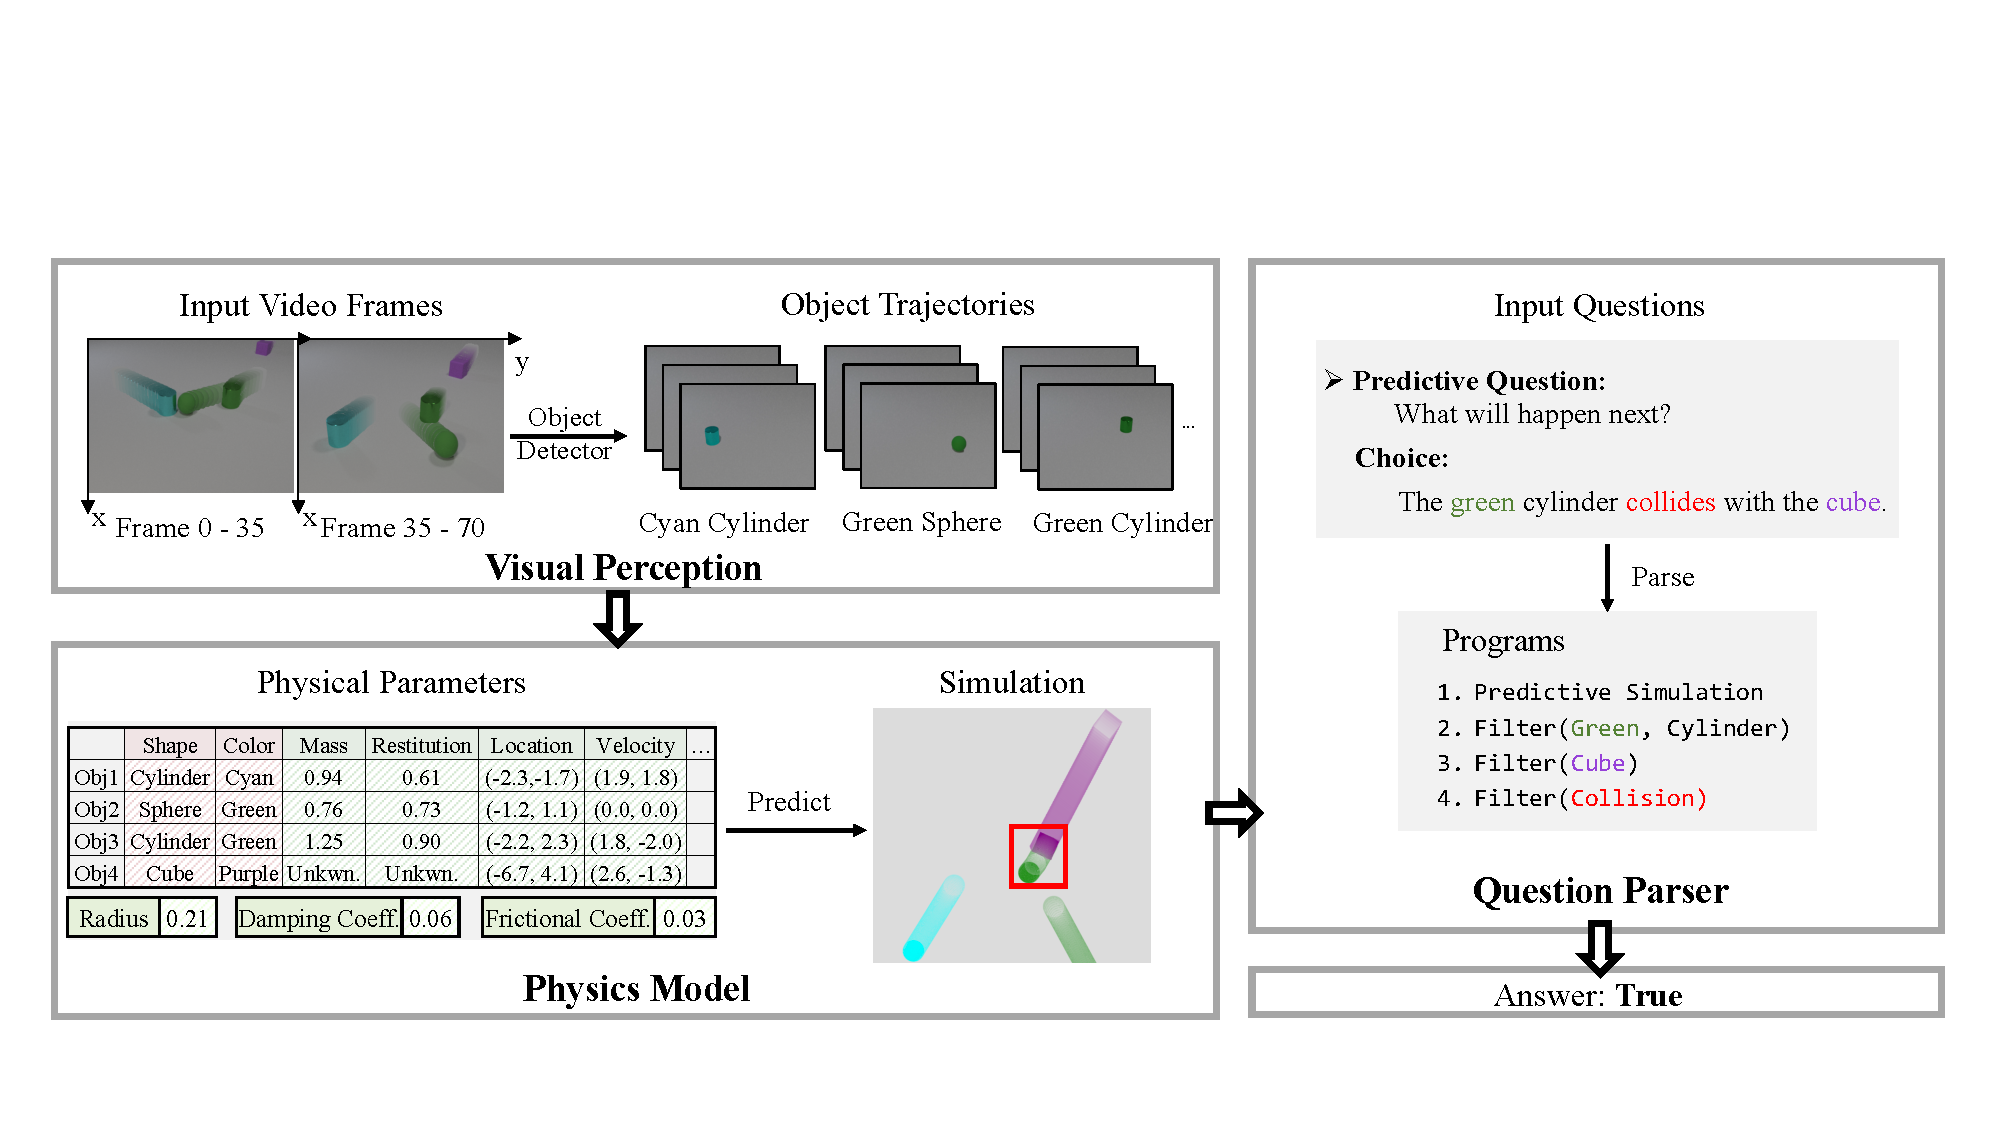
\includegraphics[width=1\textwidth]{images/overview.pdf}
        \vspace{-2em}
    \end{center}
}
\headerbox{\bf\color{blue} Concept Learning and Program Execution}{name=abstract,column=0,below=formulation,span=2}{
    \vspace{-0.3em}
    \begin{center}
        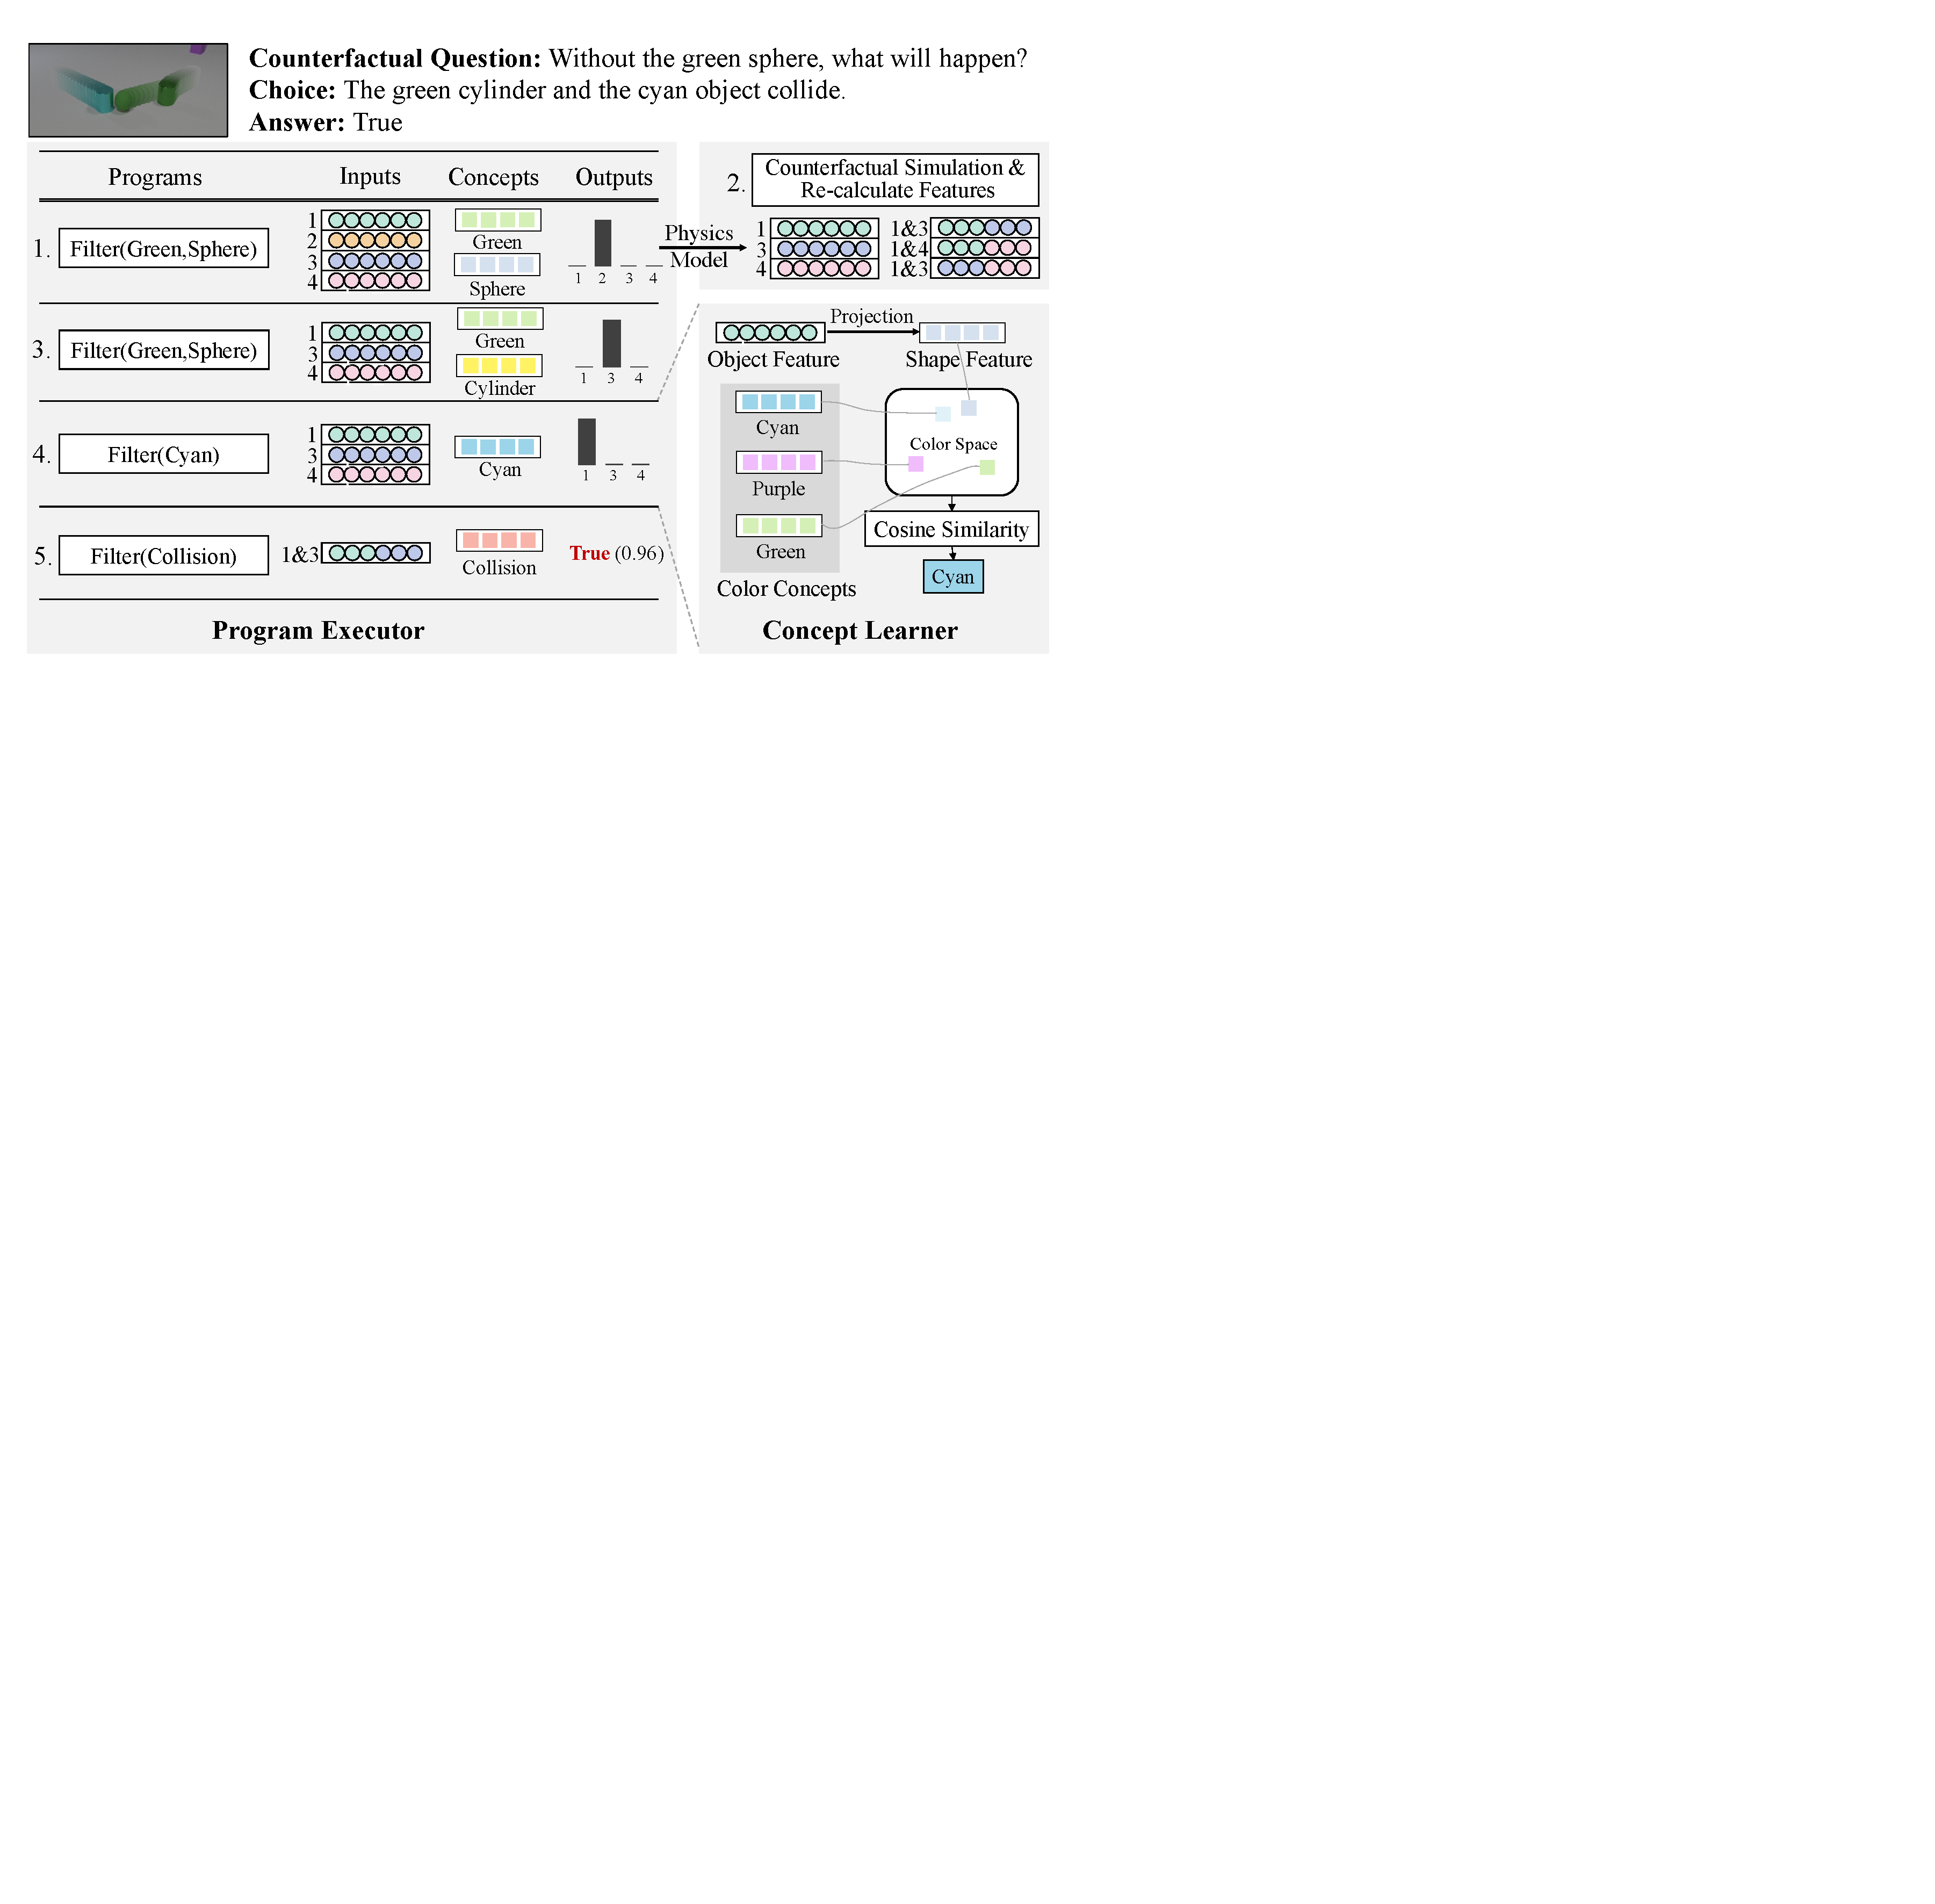
\includegraphics[width=1\textwidth]{images/illustration.pdf}
    \end{center}
}


\headerbox{\bf\color{blue} Experiments \& Results}{name=results,column=2,row=0,span=3}{
%    \begin{minipage}[t]{0.42\textwidth}
%        \textbf{\color{blue}Learning New Concepts:} 
%        \vspace{-0.8em}
%        \begin{center}
%            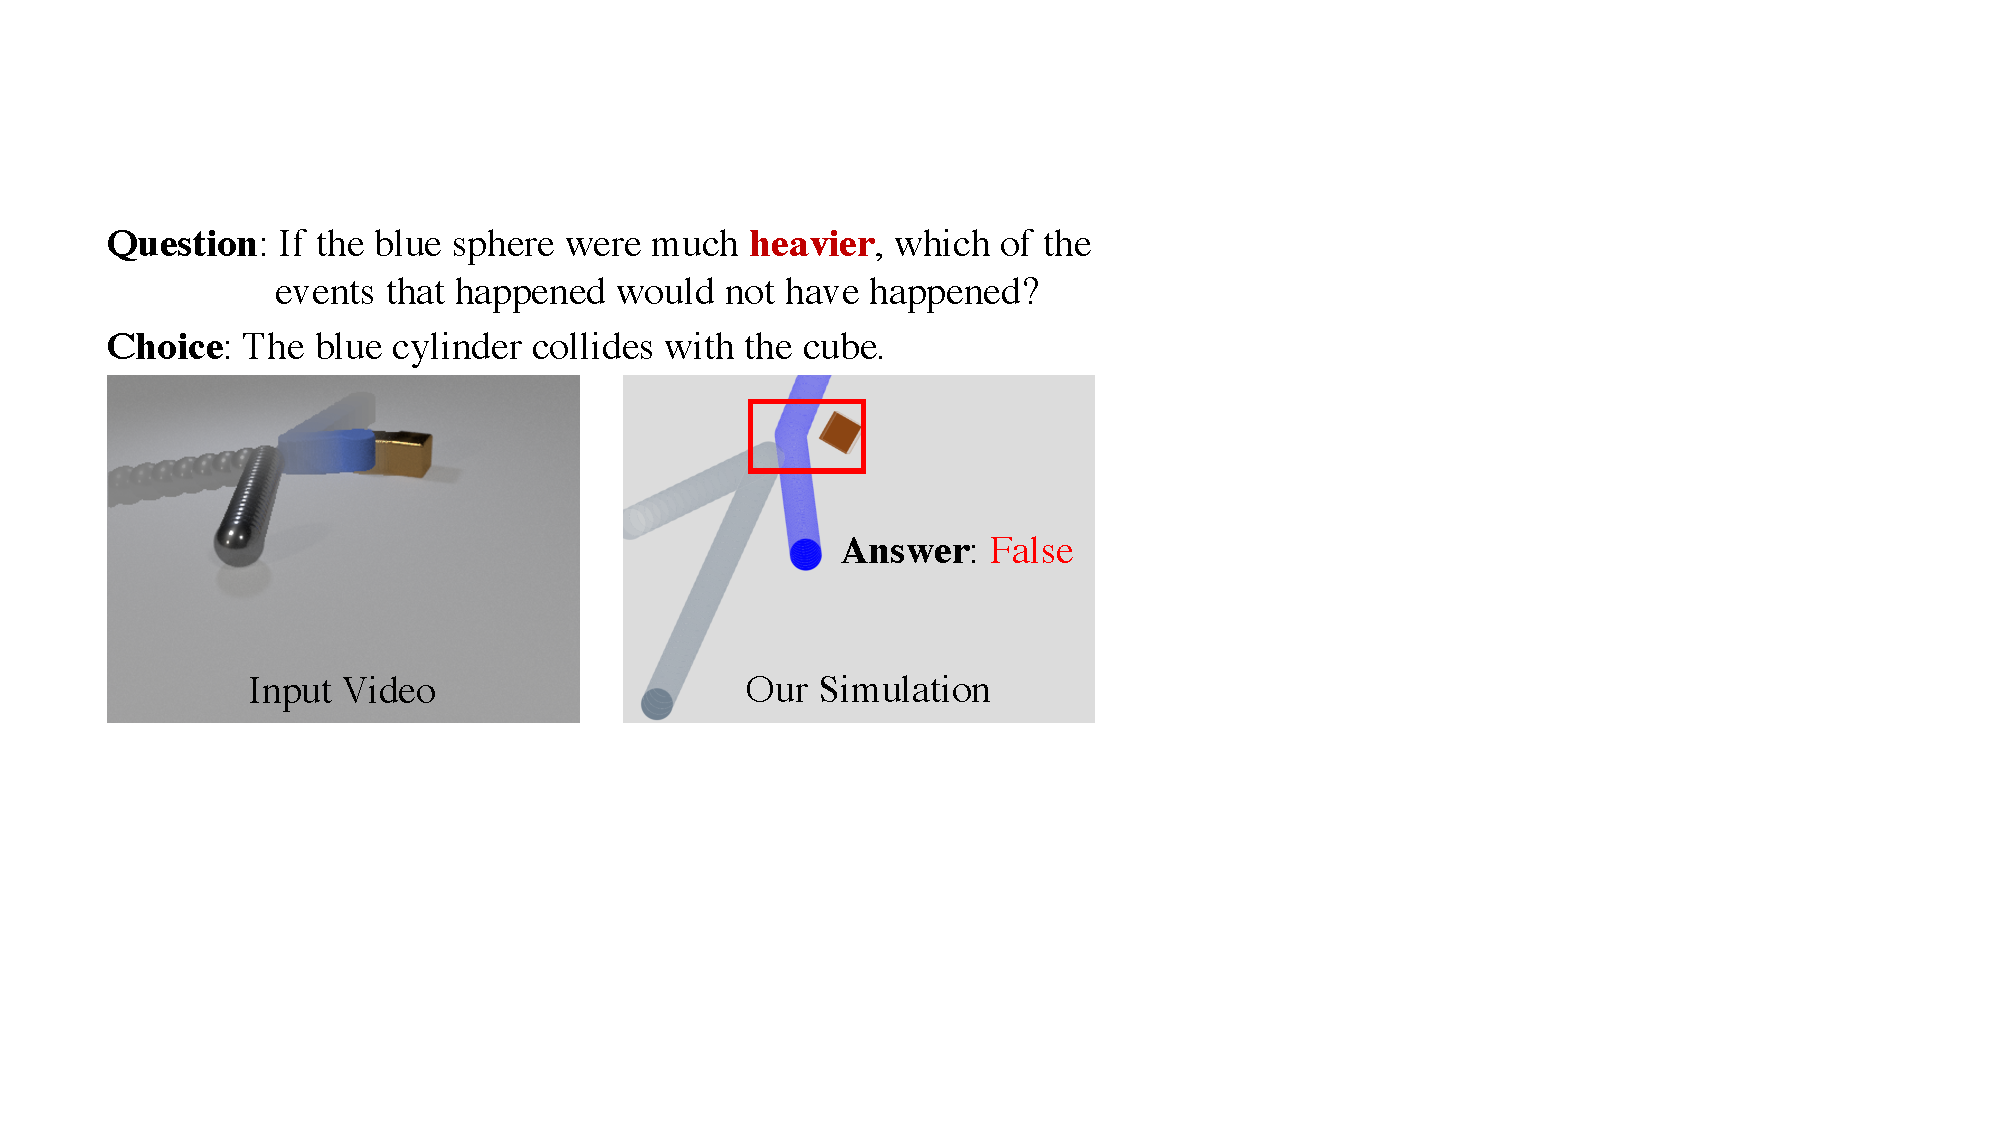
\includegraphics[width=\textwidth]{images/few-shot.pdf}
%        \end{center}
%
%%        \vspace{0.1em}
%        \textbf{\color{blue}Real-world Examples:} 
%        \vspace{-0.8em}
%        \begin{center}
%            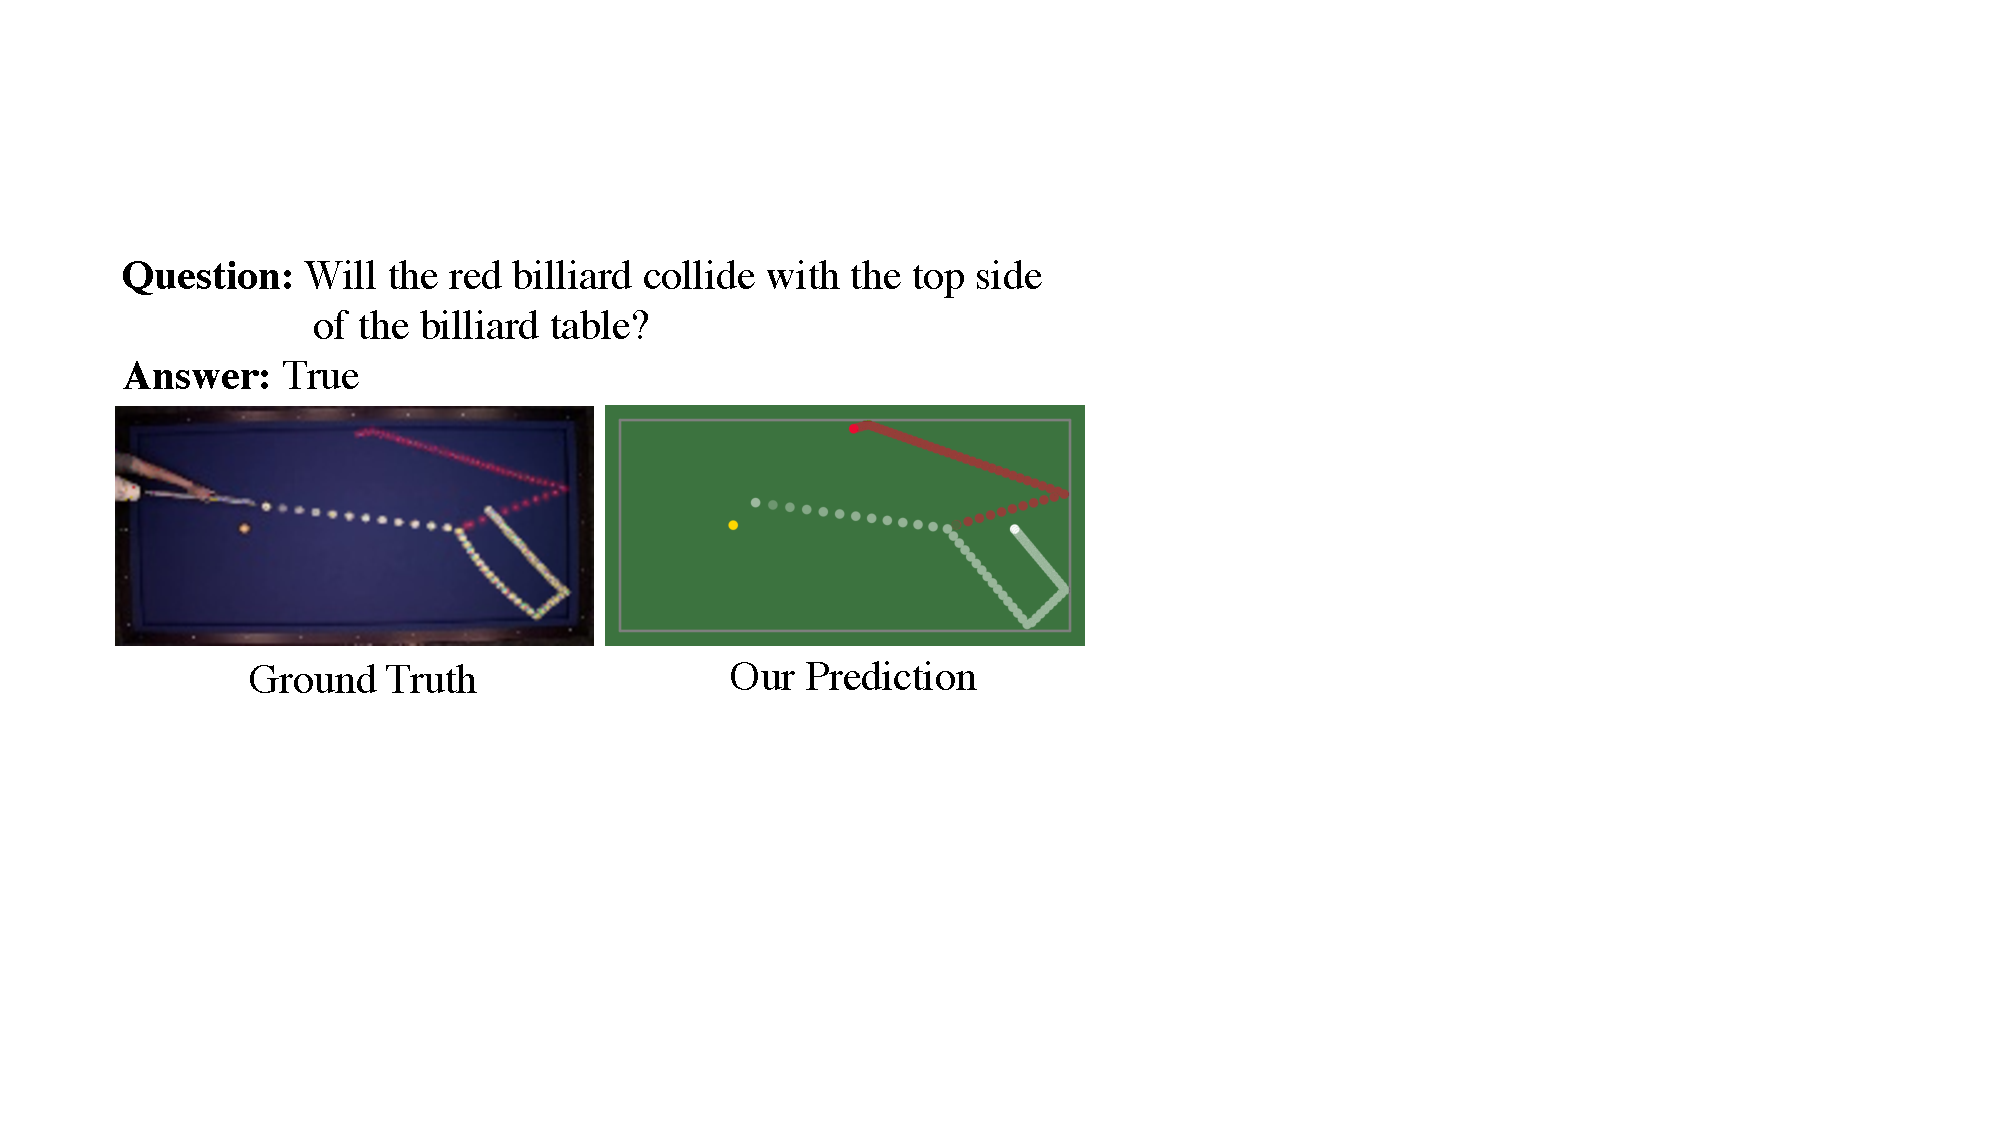
\includegraphics[width=\textwidth]{images/billiards.pdf}
%        \end{center}
%    \end{minipage}\hfill
%    \begin{minipage}[t]{0.57\textwidth}
%        \textbf{\color{blue}Results on CLEVRER Benchmark:} 
%        \vspace{-0.8em}
%        \begin{center}
%            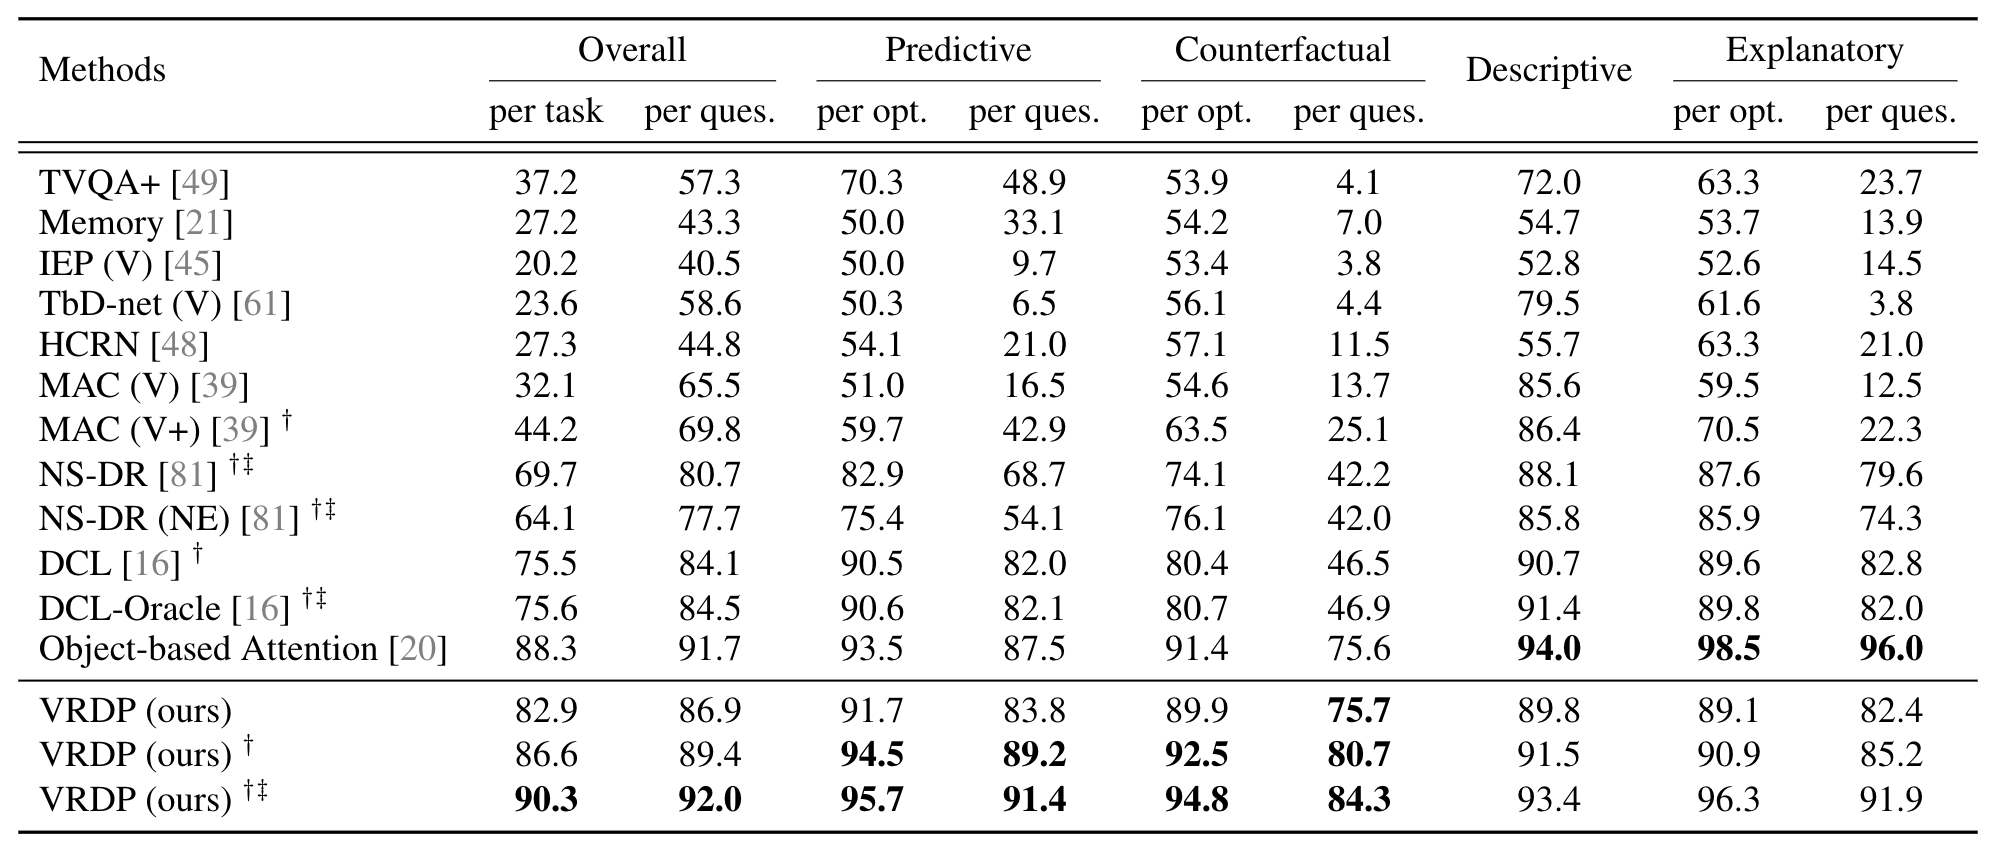
\includegraphics[width=\textwidth]{images/overall_exps.png}
%        \end{center}
%
%        \textbf{\color{blue}Data Efficiency Evaluation:} 
%        \vspace{-0.8em}
%        \begin{center}
%            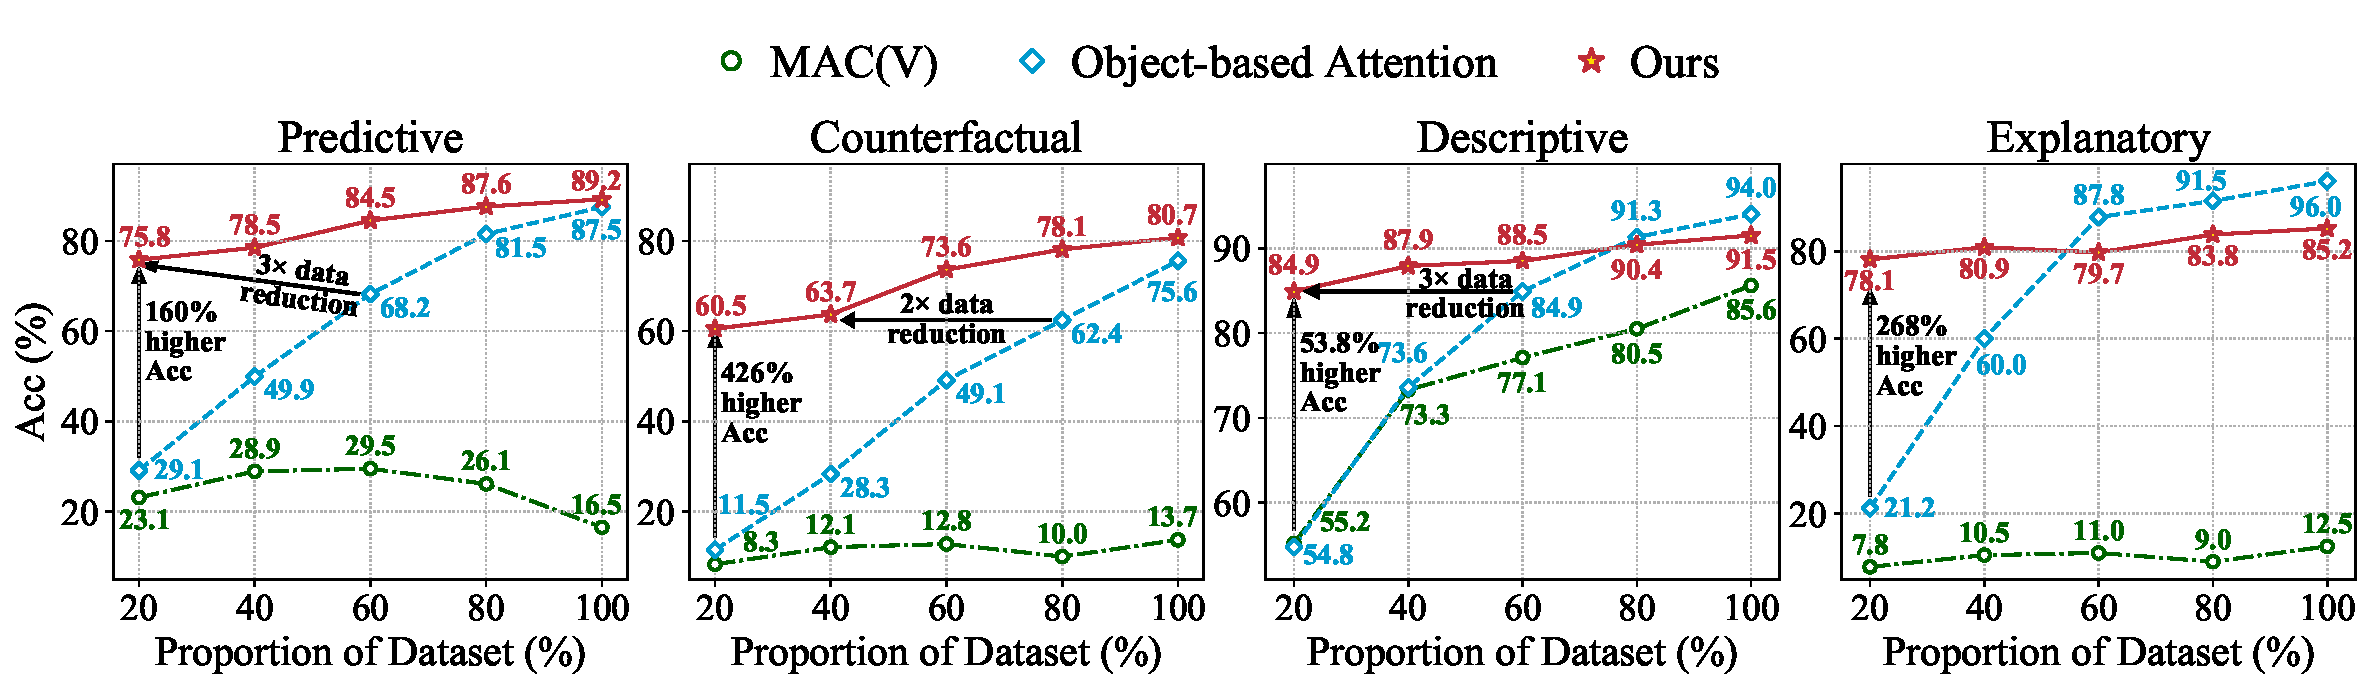
\includegraphics[width=\textwidth]{images/data_efficiency.pdf}
%        \end{center}
%    \end{minipage}

    \begin{minipage}[t]{0.37\textwidth}
        \textbf{\color{blue}Learning New Concepts:} 
        \vspace{-0.6em}
        \begin{center}
            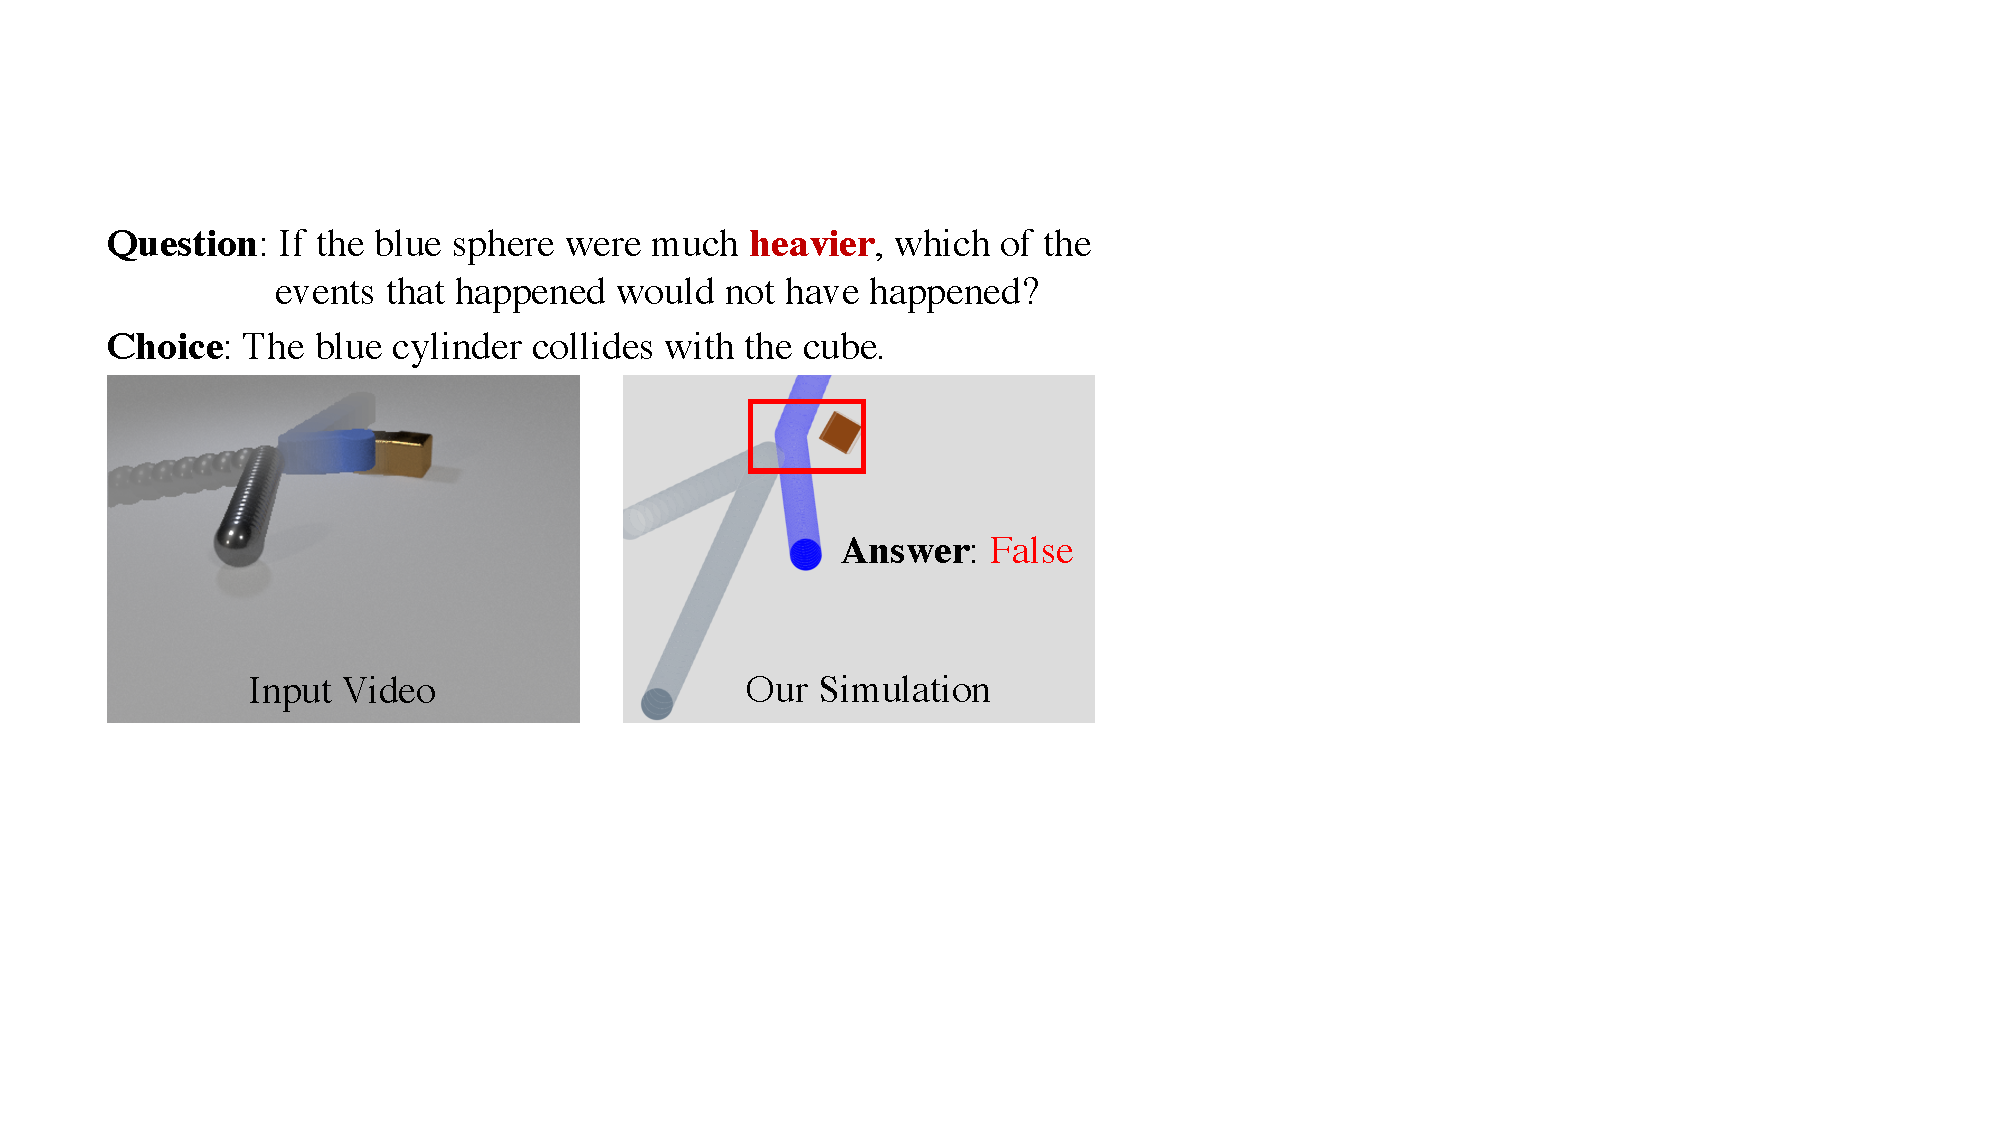
\includegraphics[width=\textwidth]{images/few-shot.pdf}
        \end{center}
        \vspace{-0.4em}
        \textbf{\color{blue}Real-world Examples:} 
        \vspace{-0.6em}
        \begin{center}
            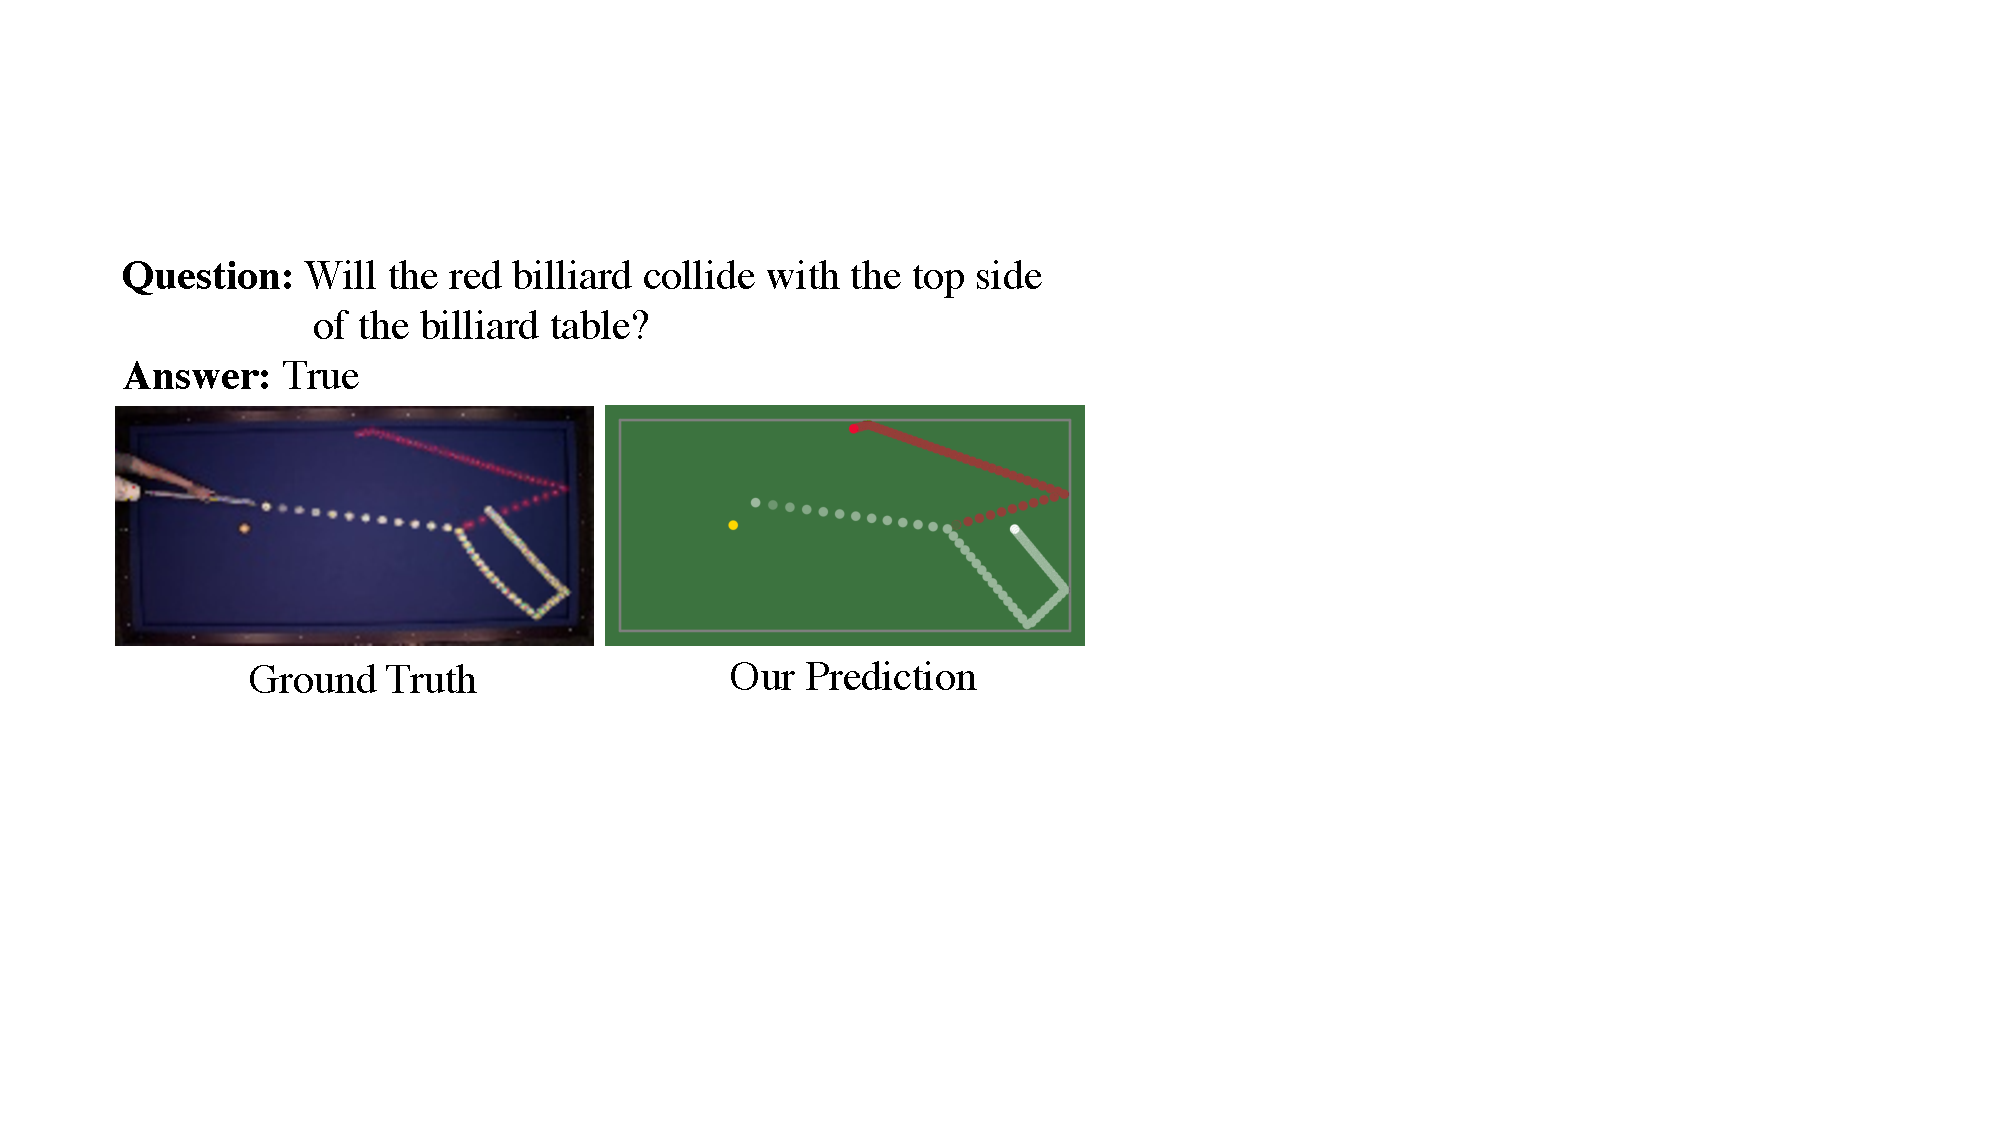
\includegraphics[width=\textwidth]{images/billiards.pdf}
        \end{center}
    \end{minipage}
    \hfill
    \begin{minipage}[t]{0.62\textwidth}
        \textbf{\color{blue}Results on CLEVRER Benchmark:} 
        \vspace{-0.8em}
        \begin{center}
            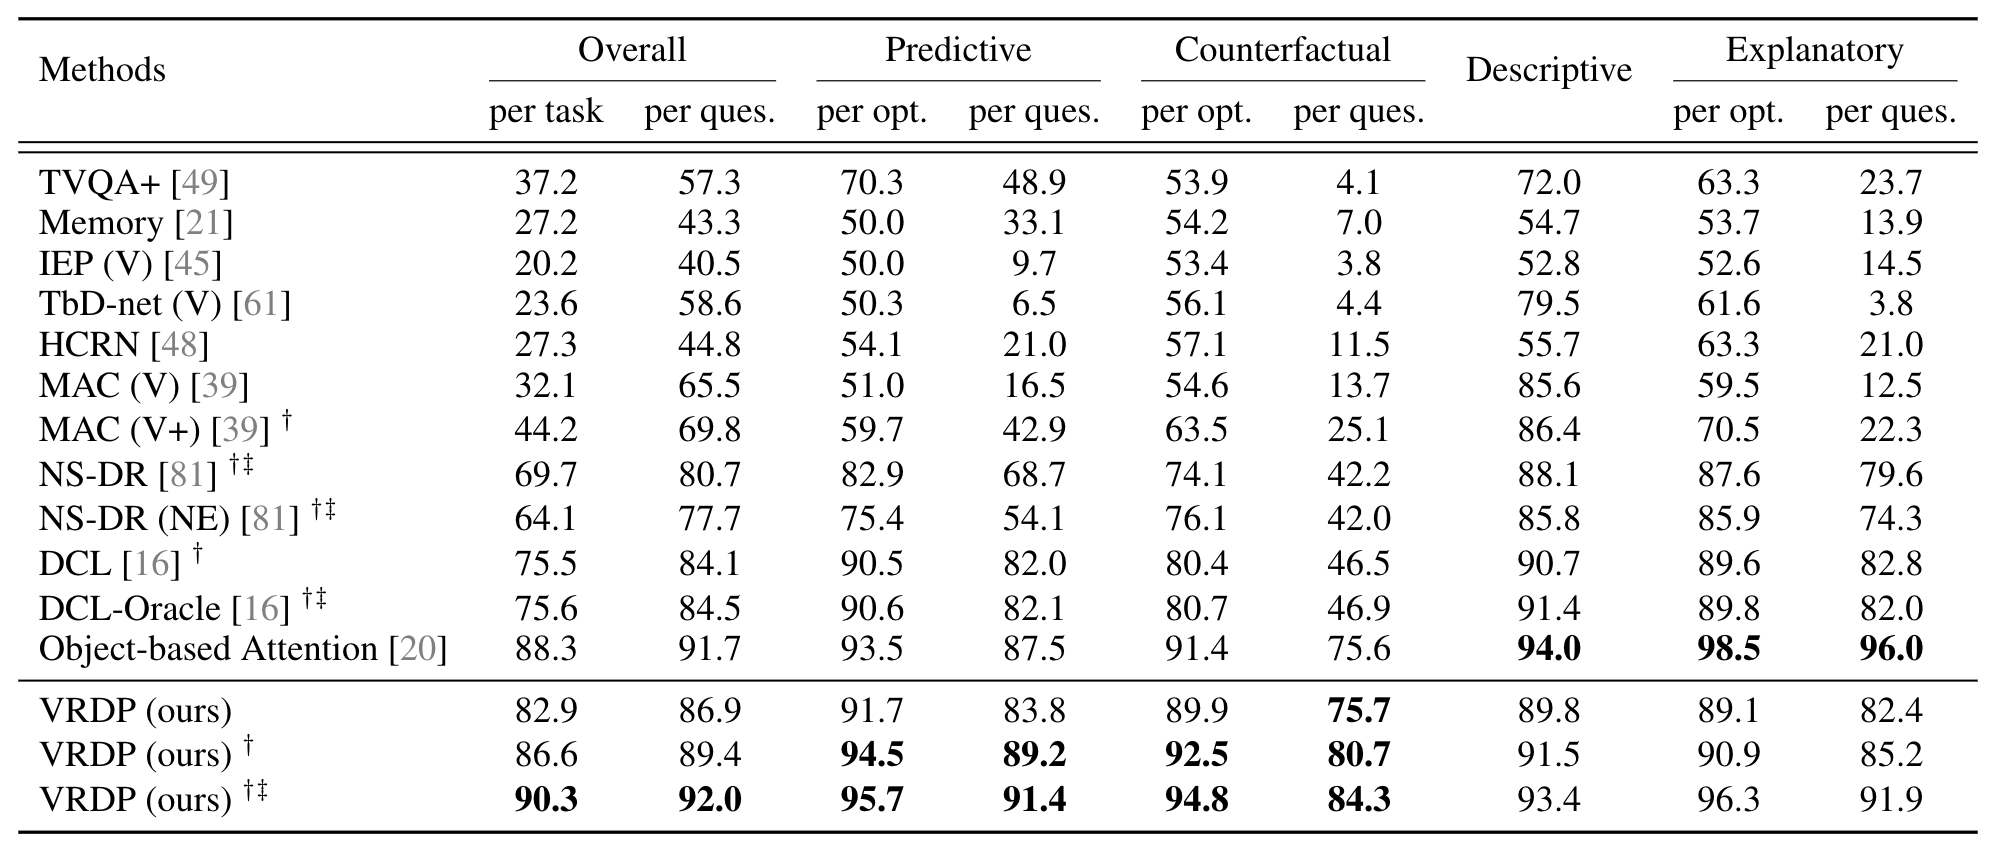
\includegraphics[width=\textwidth]{images/overall_exps.png}
        \end{center}
        \vspace{-0.4em}
        \textbf{\color{blue}Ablation Study on the Optimization of Physical Parameters:} 
        \vspace{-0.8em}
        \begin{center}
            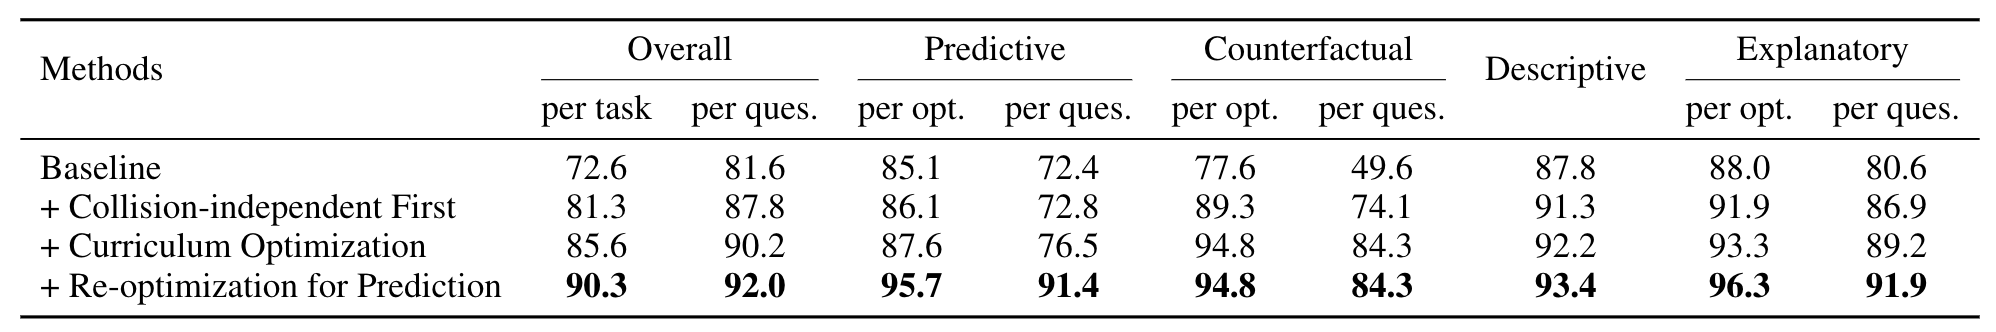
\includegraphics[width=\textwidth]{images/ablation.png}
        \end{center}
    \end{minipage}

	\vspace{0.4em}
    \textbf{\color{blue}Data Efficiency Evaluation:} 
    \vspace{-0.8em}
    \begin{center}
        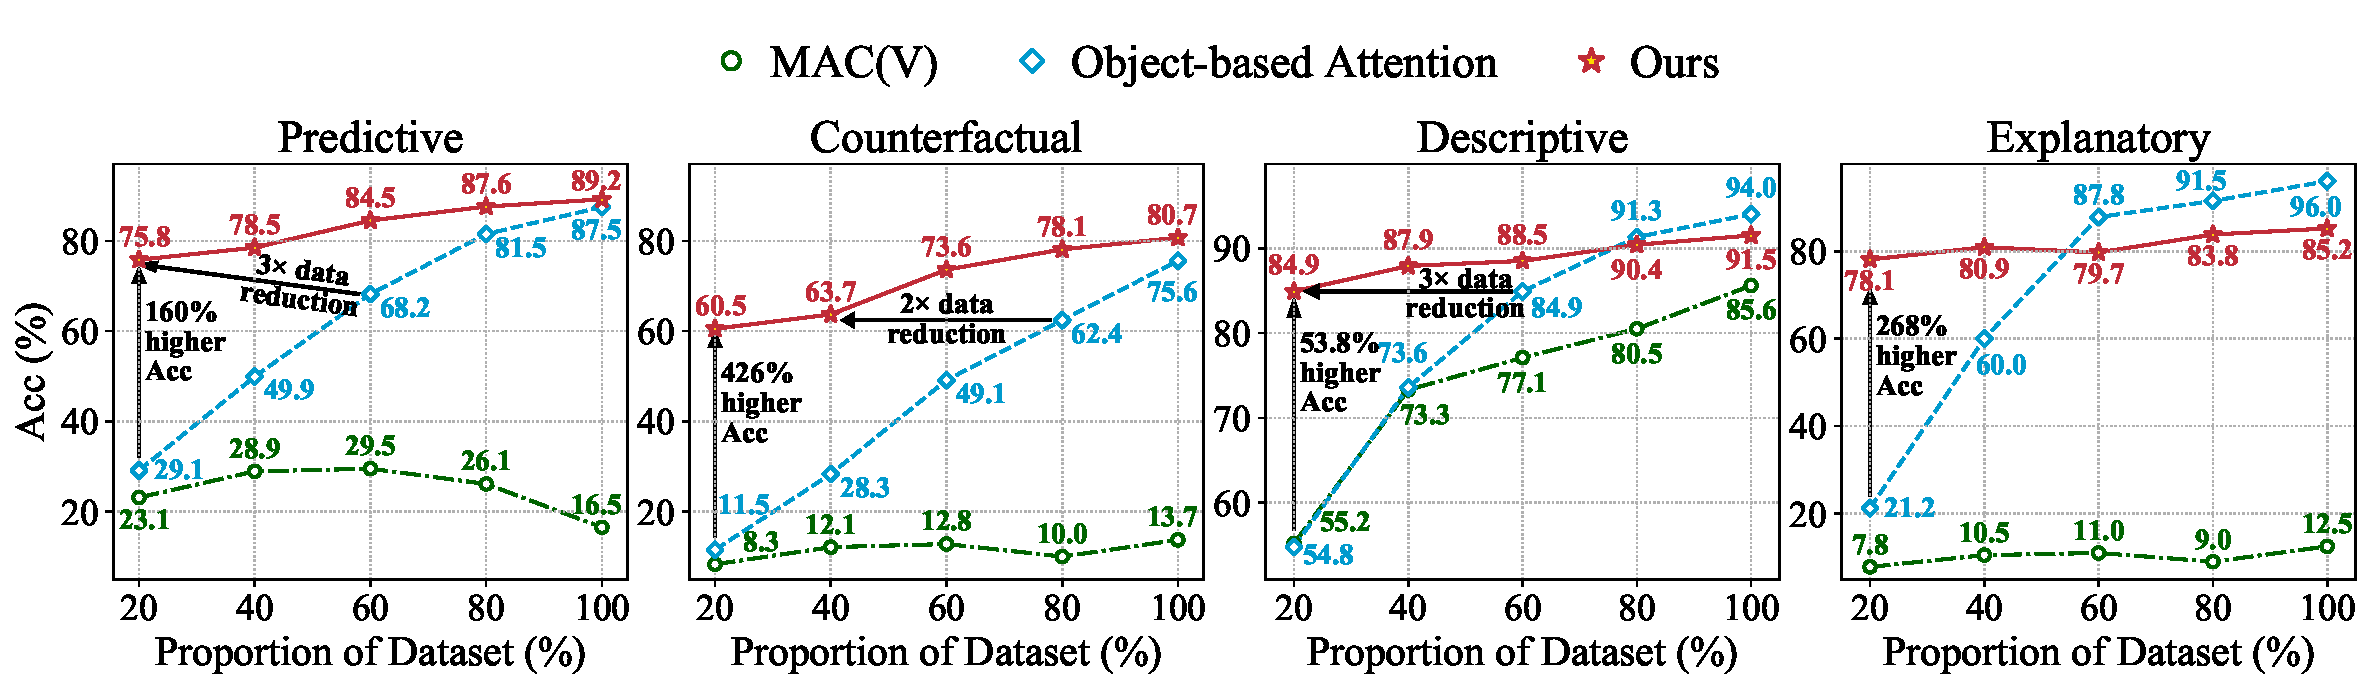
\includegraphics[width=0.92\textwidth]{images/data_efficiency.pdf}
    \end{center}
	
    \vspace{-0.8em}
    \begin{minipage}[t]{0.49\textwidth}
        \textbf{\color{blue}Examples on the CLEVRER dataset:} 
        \vspace{-0.8em}
        \begin{center}
            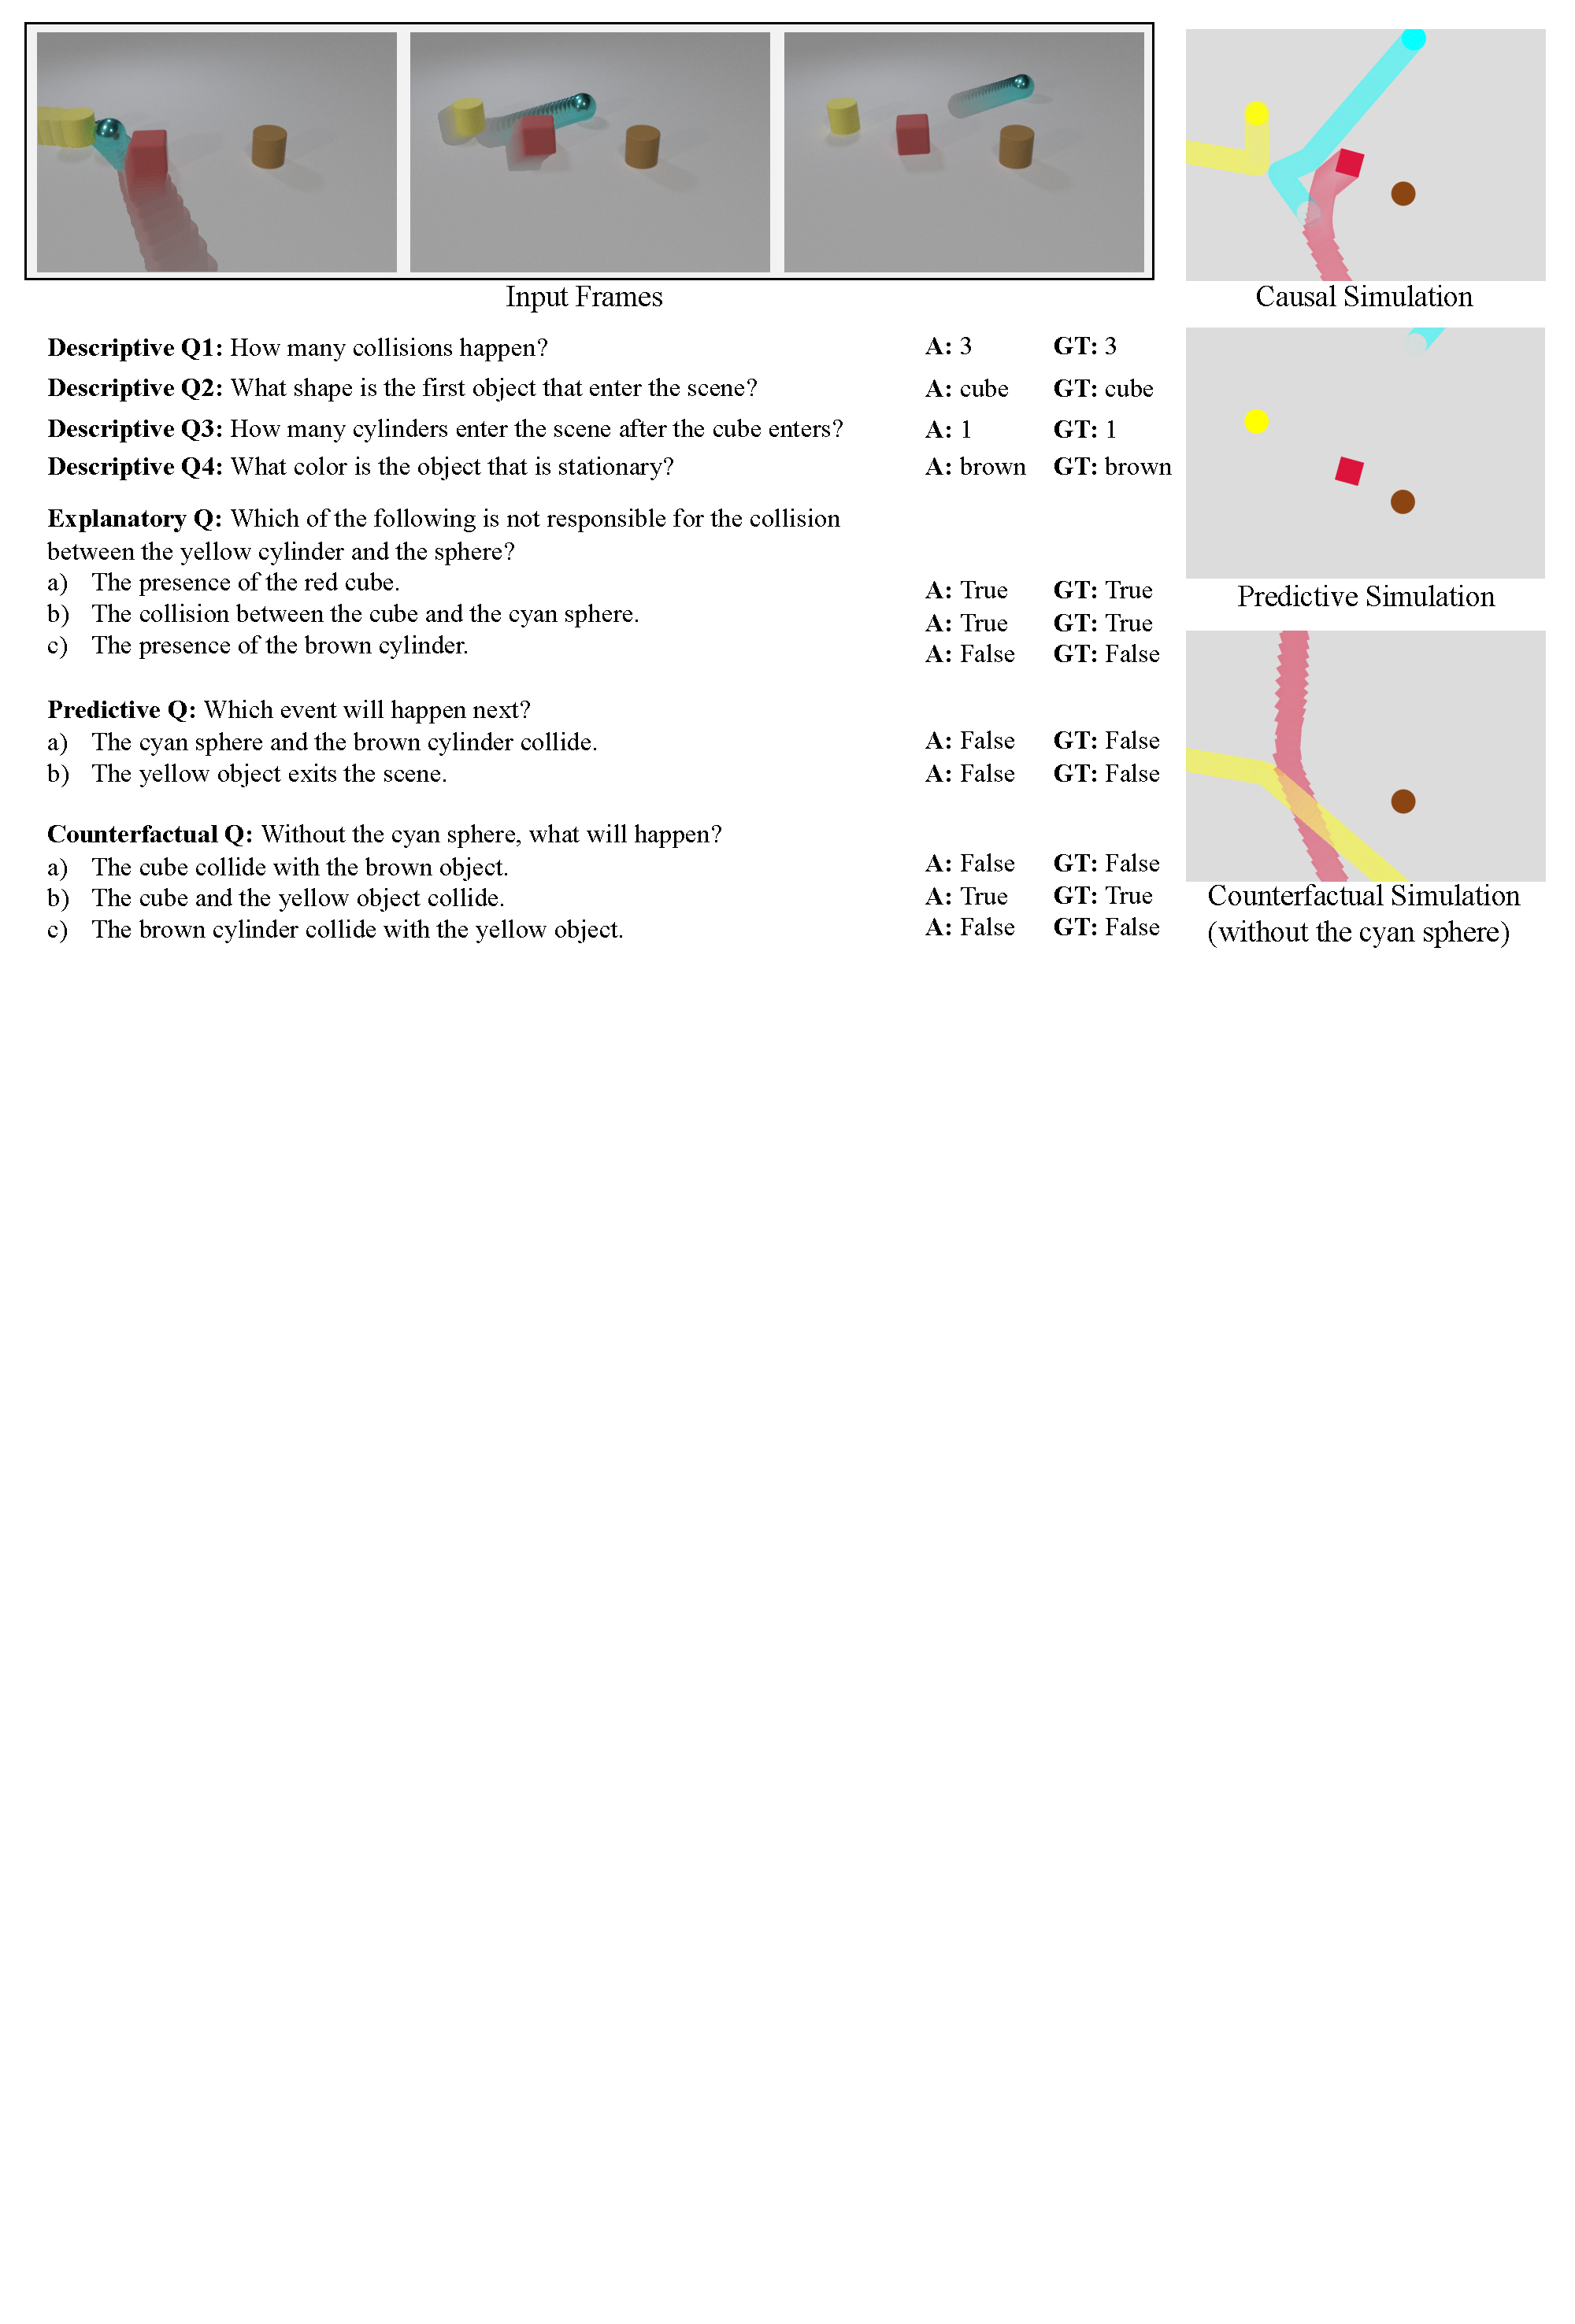
\includegraphics[width=\textwidth]{images/visualize_7.pdf}
        \end{center}
    \end{minipage}\hfill
    \begin{minipage}[t]{0.49\textwidth}
        \textbf{\color{blue} } 
        \vspace{-0.8em}
        \begin{center}
            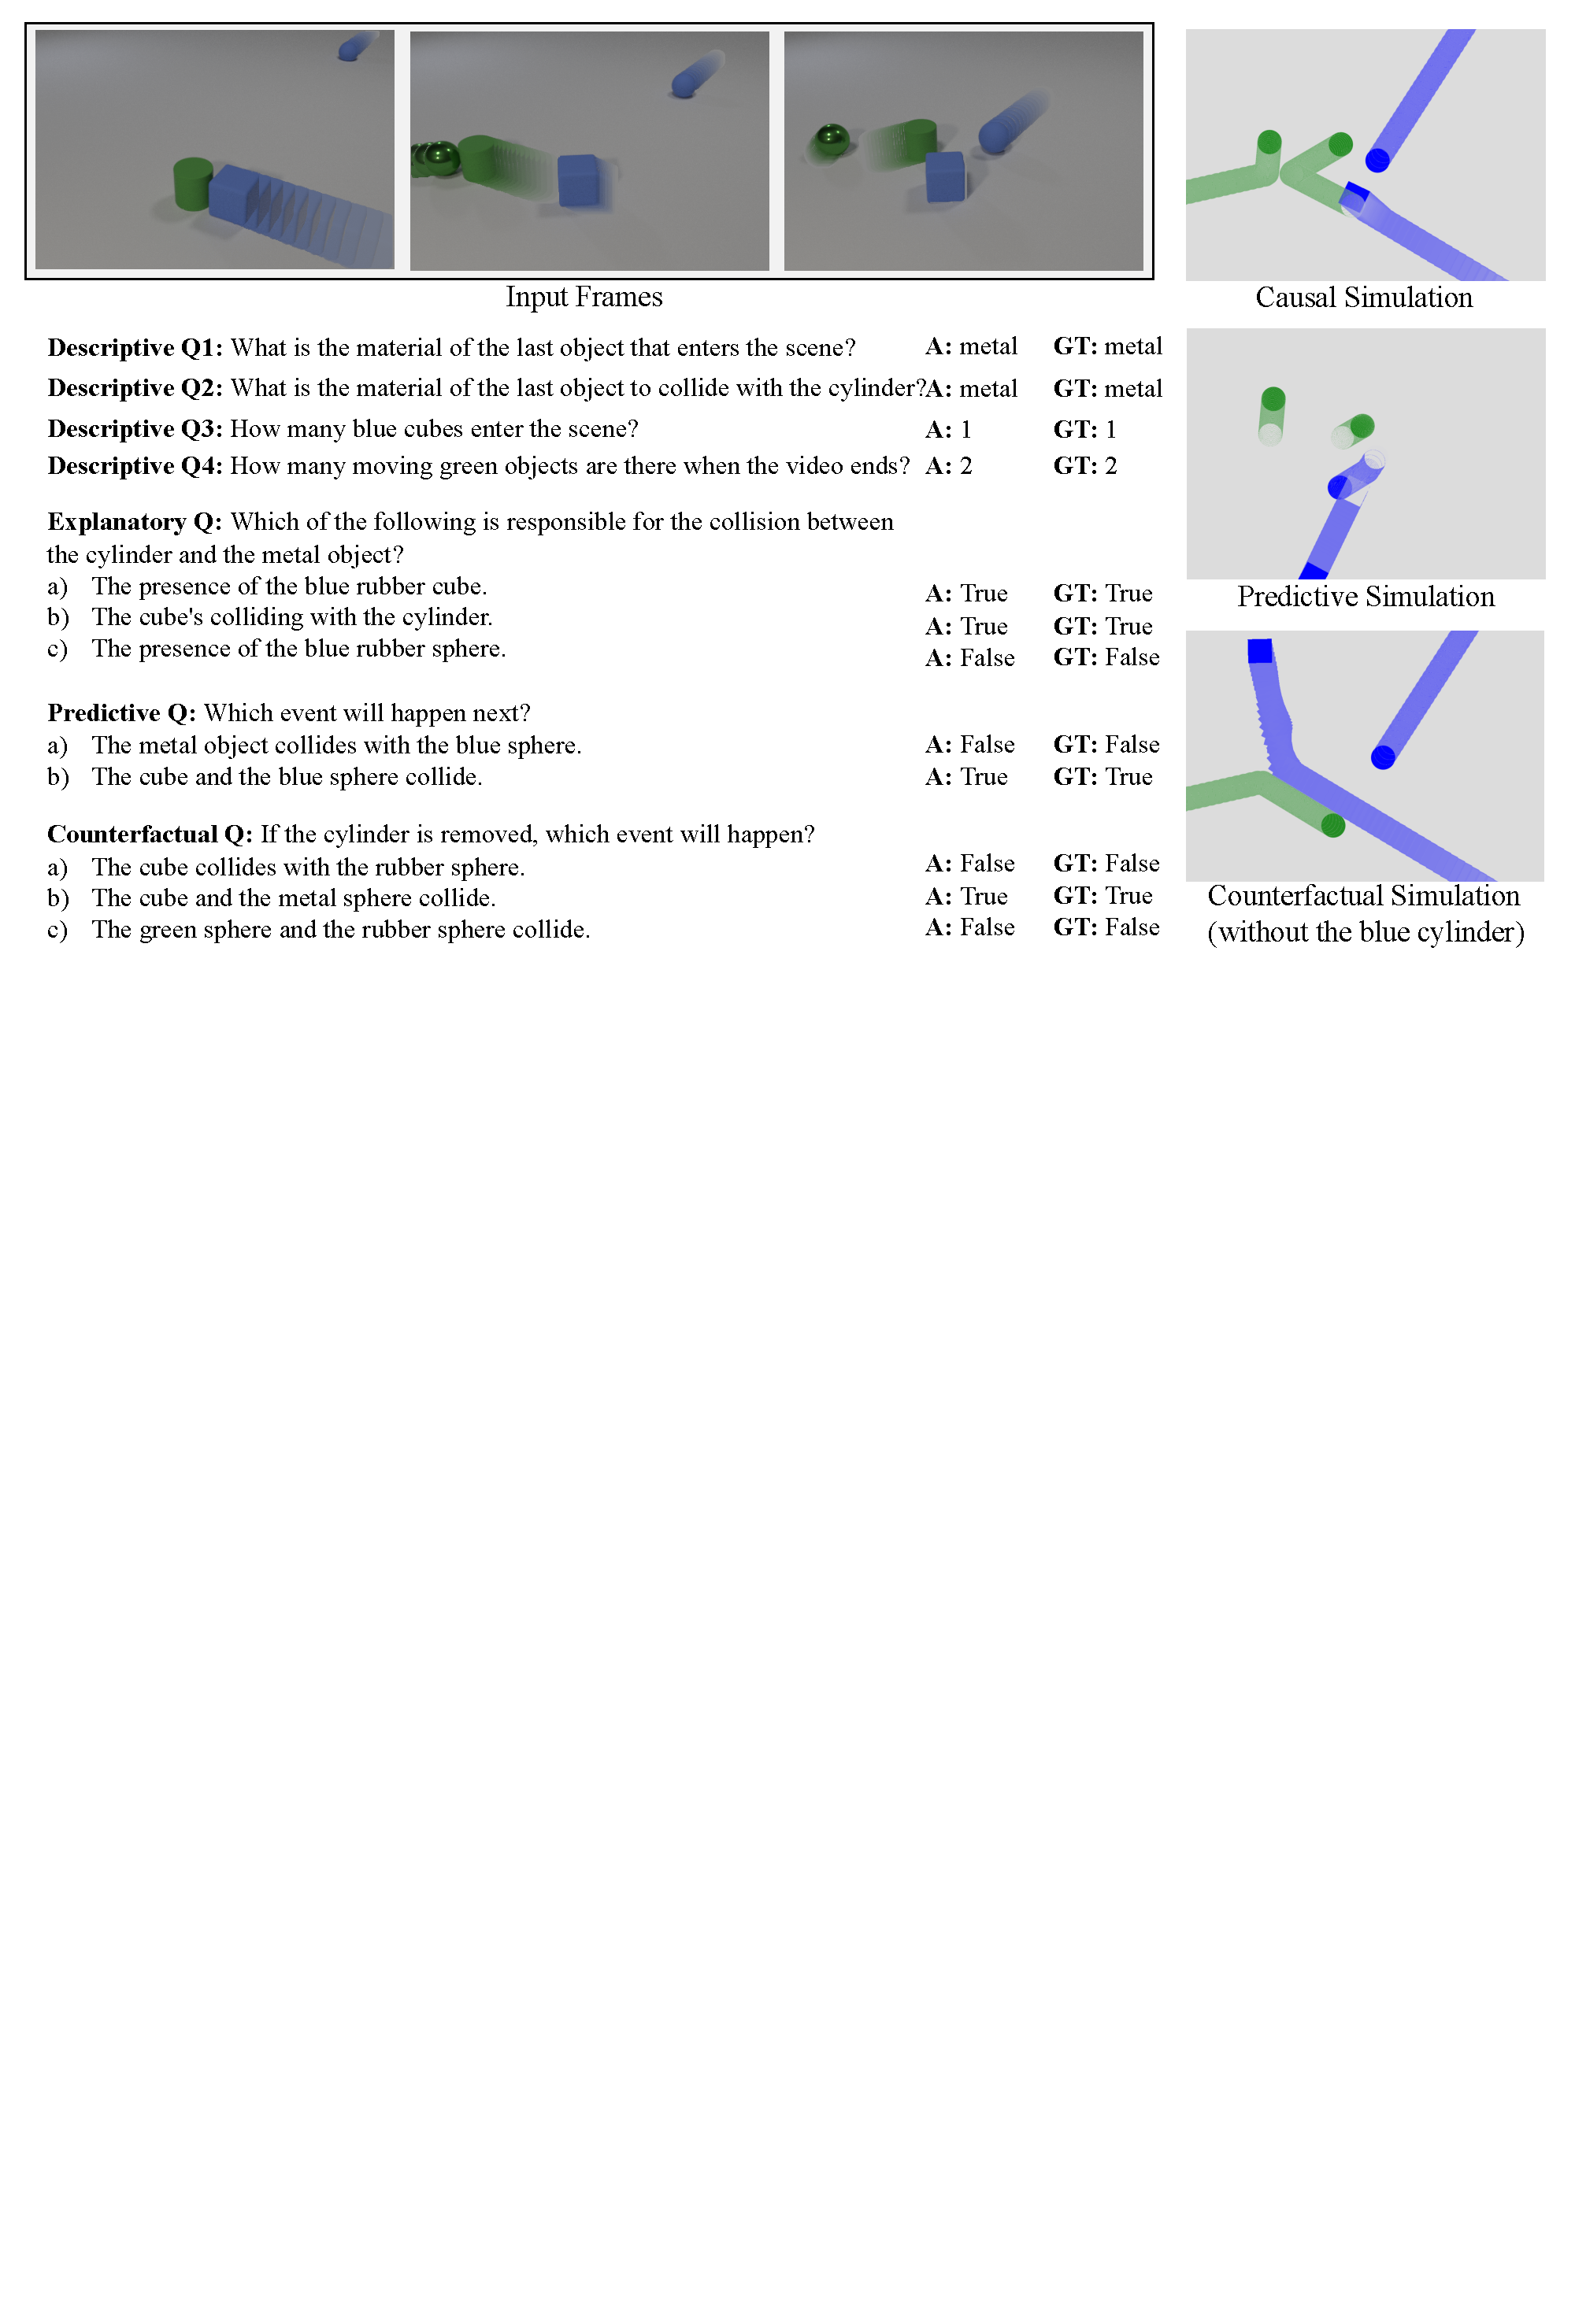
\includegraphics[width=\textwidth]{images/visualize_210.pdf}
        \end{center}
    \end{minipage}


%    \begin{minipage}[t]{0.72\textwidth}
%        \textbf{\color{blue}Qualitative Results on :} \\
%        \vspace{-1.5em}
%        \begin{center}
%            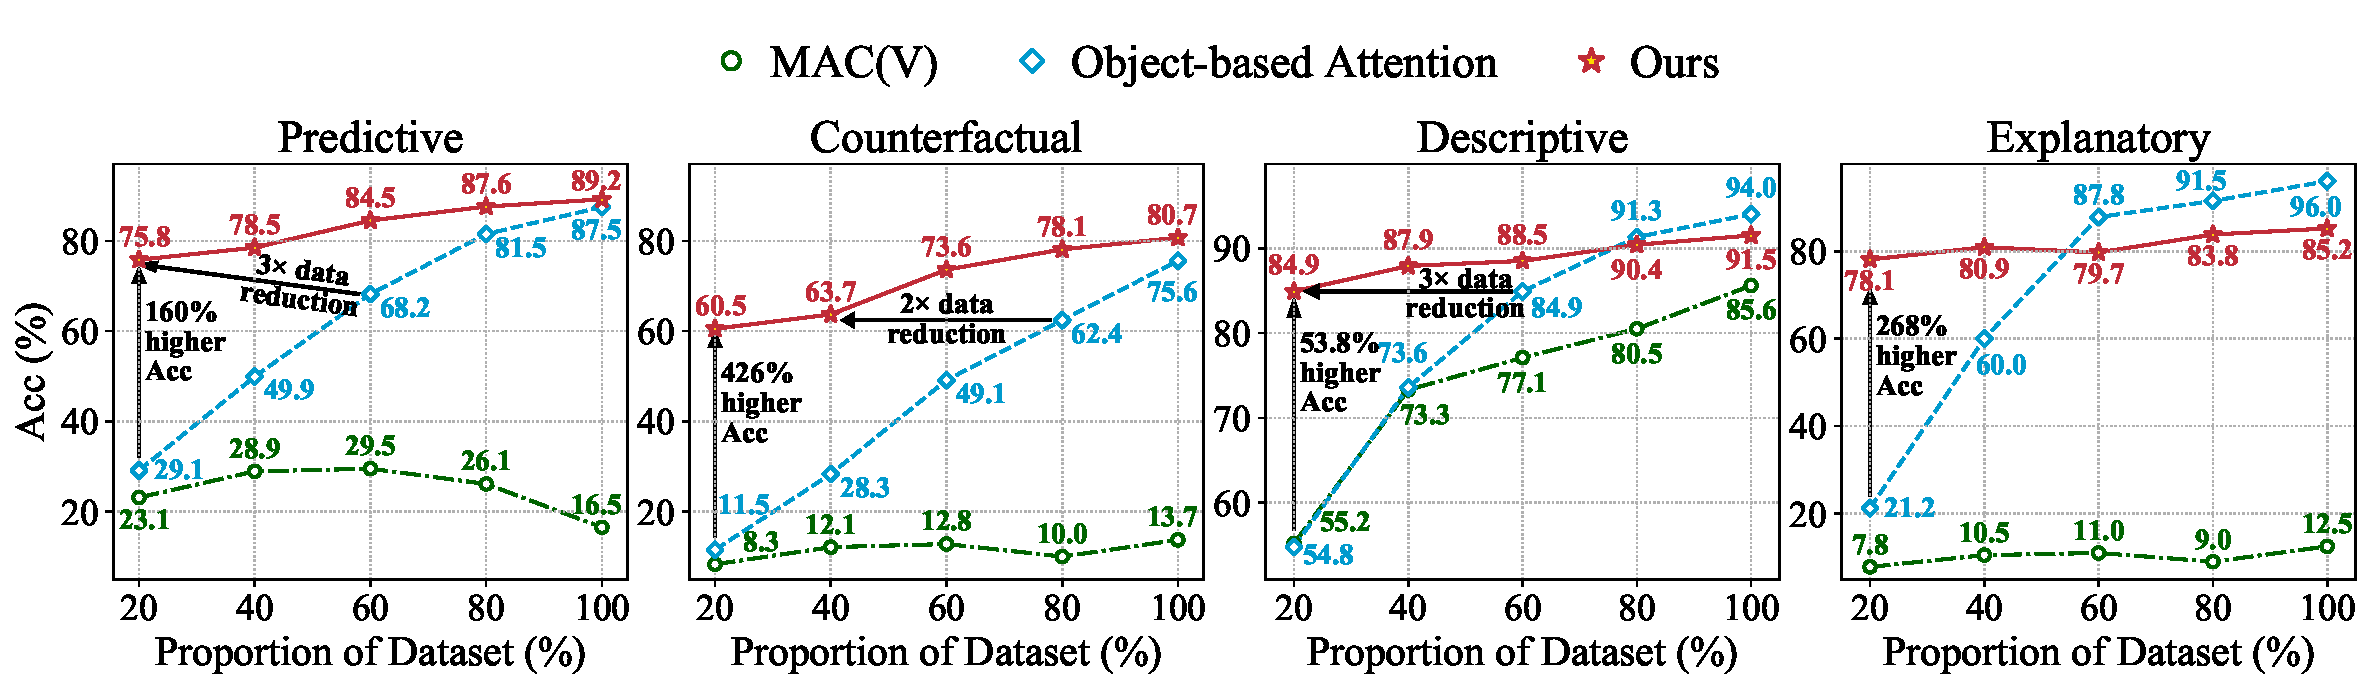
\includegraphics[width=\textwidth]{images/data_efficiency.pdf}
%        \end{center}
%    \end{minipage}
%    \begin{minipage}[t]{0.28\textwidth}
%    \textbf{\color{blue}References:} \\
%        \vspace{-1.0em}
%        \begin{enumerate}[label={[\arabic*]}]
%            \footnotesize
%            \item UPS-FCN [Chen~\emph{et al.}, ECCV8]
%            \item DiLiGenT [Shi~\emph{et al.}, TPAMI19]
%            \item AM07 [Alldrin~\emph{et al.}, ICCV07]
%            \item SM10 [Shi~\emph{et al.}, CVPR10]
%            \item WT13 [Wu and Tan, CVPR13]
%            \item LM13 [Lu~\emph{et al.}, CVPR13]
%            \item PF14 [Papadhimitri and Favaro, IJCV14]
%            \item LC18 [Lu~\emph{et al.}, TPAMI18]
%            \item L2 [Woodham, OE1980]
%            \item IS18 [Ikehata, ECCV18]
%            \item Gourd\&Apple [Alldrin~\emph{et al.}, CVPR08]
%            \item Light Stage [Einarsson~\emph{et al.}, EGSR06]
%        \end{enumerate}
%    \end{minipage}
}
\end{poster}
\end{document}
